\chapter{Aims and objectives}
\label{chap:aim}
%Aims describe what you want to achieve. Objectives describe how you are going to achieve those aims.

Poor motor performance skills can be an indicator for various development delays such as Autism Spectrum Disorder (ASD).
ASD is a disorder that has been increased in the population in the last years. The main reason for that is that methods for discover ASD has been improved and knowledge about the disorder has expand and child care personnel has been educate to look for symptoms in early stage of the child's development. %(https://www.fhi.no/fp/barn-og-unge/utviklingsforstyrrelser/autisme---faktaark/)
Various research has been done to highlight methods (reference) discovering ASD and to emphasize ASD therapy possibilities. Nowadays, standard evaluation tests for instance, M-ABC2, MOT4-5, BOT2 are used by psychologist in order to determine development delays.%(Reference: http://entwicklungsdiagnostik.de/m-abc-2.html)
Tests such as M-ABC2, evaluate children's motor-coordination skills. Their test methods focus on evaluating of hand dexterity, balance and ball skills. Furthermore, research showed that children with ASD have disruption of normal movement pattern which also is an indication of motor coordination deficit.(reference). However, according to (reference), test methods that could determine ASD are expensive, time consuming and demand a laboratory environment. A Laboratory is an artificial environment where indeed influencing factors can be controlled but on the other hand such environments can also affect children's behavior. Some become uncomfortable and insecure which in worst case, distort the result. (find REFERENCE) For that reason, the aim of this project is to investigate whether mobile sensors such as Leap Motion and gesture interaction could be used as a supplementary evaluation and screening tool for motor development delays. Furthermore, the research will show if this is a convenient measurement tool to determine ASD in an early stage. The benefits of using Leap Motion are many, as for instance the portability and low acquisition cost. The evaluation can happen anywhere, even in an environment where kids feel comfortable and familiar. Leap Motion is a sensor for gesture controlled interfaces. Nowadays, evaluation exercises are more or less analogical, (interview) as described in “Entwicklingsdiagnostik”. %(http://entwicklungsdiagnostik.de/m-abc-2.html) 
However, a digital evaluation tool could be more appealing to the contemporary technological standard. Since Leap motion is able to screen fine-motor movements, it would be a suitable evaluation tool which is enjoyable, accessible and economical.

%sløyfe denne setningen?
Moreover, the Leap motion sensor may not only be a usefully screening tool but it might be used as a therapy tool for fine motor exercises as well.

%objects -  how to achieve aims
%create a system
%do an experiment

In order to achieve the aim of this project a concept needed to be created and tested. This concept had to fulfill the requirements of the Leap Motion sensor and gesture interaction and also address various parameters. As mentioned in section \ref{sec:asd}, ASD is defined by several deficits such as motor-coordination deficit, sensory-motor deficit, motor-timing disruption, psycho-motor deficit, etc. These parameters are en essential brick for this concept.

A software game is a convenient approach to combine sensor and gesture interaction. This concept would have several modules in order to satisfy various parameters. About 5 modules or less would be enough to checks the capacity of motor coordination and hand dexterity. An example of modules which could be suitable for this concept is described below:  

\vspace{5mm} %5mm vertical space
\hfill \break
Module 1 - Ladybug\newline
Task description: The goal of this task is to put as many ladybugs on a three a possible in a certain time frame. The child has to move a ladybug from the ground up to the tree by only his/her index finger.
Evaluation parameters: count the amount of bug are move in a given time period
Based on: M-ABC2 ( insert coins task)
\vspace{5mm} %5mm vertical space
\hfill \break
Module 2 - Flying balloon\newline
Task description: Flying balloon is a pointing game where the participant must hit the balloons in order to burst them. The balloons are moving over the screen entirely arbitrary. The goal is to burst as many balloon as possible in a certain time period.
Evaluation parameters: Hand eye coordination, accuracy and timing
Based on: M-ABC2 
\vspace{5mm} %5mm vertical space
\hfill \break
Module 3 - Mole in the hole\newline
Task description: The goal of this game is to guide the mole out of his hole. This is a precision game which demands concentration and patience 
Evaluation parameters:  precision, concentration, patience 
Based on: M-ABC2 for hand dexterity test - trace a track
\vspace{5mm} %5mm vertical space
\hfill \break
Module 4 - MEMO \newline
Task description: The game builds on the participants memory ability.  The participant will see a row of objects and the corresponding gestures for a certain amount of time. The participant has to memorize the gesture belonging to the object. Than the object appears on the screen and the participant has to remember the appropriate gesture. 
Evaluation parameters: remember and recall. This is a cognitive task for testing of psychomotor deficit.
Based on:
\vspace{5mm} %5mm vertical space
\hfill \break
Module 5 - Freehand drawing\newline
Task description: In this game the participant is asked to draw a shape with a the pointing finger.  The participant will see a shape on the screen and needs to repeat the drawing. The participant could also be ask to make an existing shape smaller or bigger by pinch movements.
Evaluation parameters: fine motor coordination
Based on standard tool: DMB ( trace geometrical forms) and LOS ( paint circles in the air)

%\vspace{5mm} %5mm vertical space
%\hfill \break
%To sum up autism is defined by:
%\begin{itemize}
 %   \item Motor-coordination deficit
  %  \item Sensory deficit
  %  \item Motor-timing disruption
  %  \item Psycho-motor deficit
  %  \item Disruption of normal movement pattern
%\end{itemize}


%\begin{center}
%\begin{tabular}{|c|c|c|c|c| }%| m{1cm}| m{1cm} |  m{1cm} | %m{1cm} | m{1cm}|} 
% \hline
% Parameters - identify ASD & Task description & Deficit/
%Disruption & LM parameters &  Game/task \\ 
% \hline
% \hline
% cell7 & cell8 & cell9 & cell8 & cell9 \\ 
% \hline
%\end{tabular}
%\end{center}

\begin{figure}[!ht]  %t top, b bottom, p page | you can also use h to try to get the figure to appear at the current location
  
  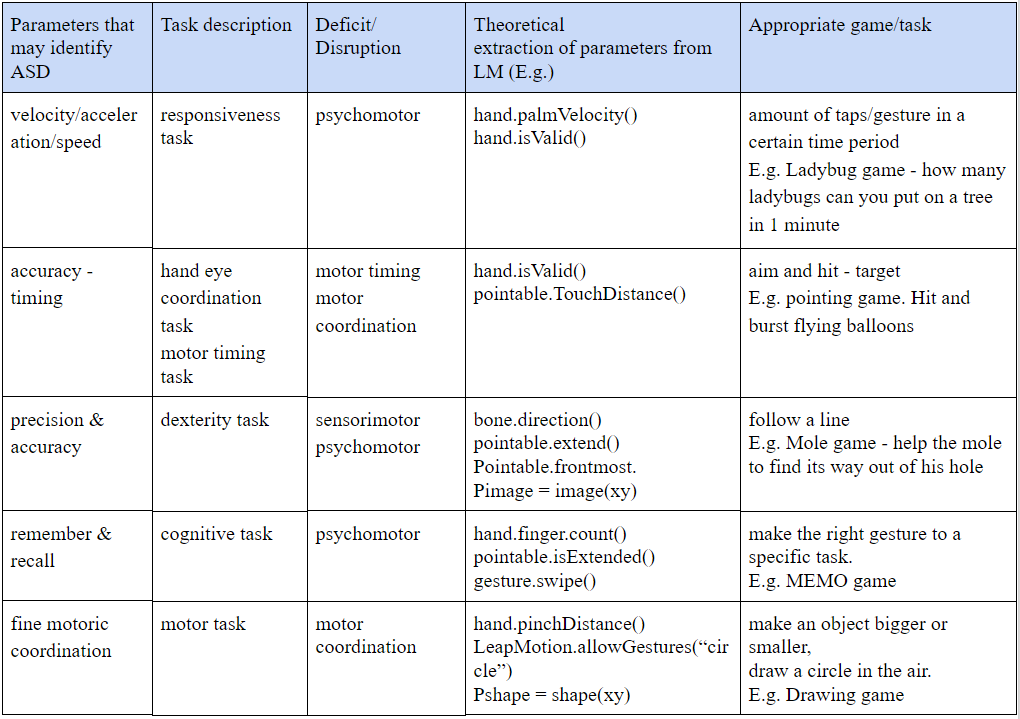
\includegraphics[width=1\textwidth]{figures/tableOfModules.png}
  \caption[Parameters and Modules.]{Parameters and Modules.}
  \label{fig:tableOfModules}
\end{figure}

\vspace{50mm} %5mm vertical space
\hfill 
\break
\section{Research Question and hypothesis}
\label{sec:researchquestion}
Defining the research question and formulating the associated hypothesis is the point of departure for all kind of research in order to find an answer of a specific problem.
\newline
The purpose of this project is to investigate if a sensor device such as Leap Motion in conjunction with gesture interaction can be used to extract parameters that could provide information about motor performance in children. The initial assumption for this project is defined and represented below. Three research question are formulated in order to explore the problem in detail.
\vspace{3mm} %vertical space
\hfill \break
%\newline
%\newline
%\textbf{RQ\texttt{\#}1:} Is it possible to extract parameters for fine-motor performing skills by using Leap Motion.
\textbf{Research Question 1:}\newline
\textbf{How can a Leap Motion controller be employed to extract parameter that measures fine-motor performance skills in children?}
\newline
By exploring the feasibility of measuring motor performance skills of children with the Leap Motion controller, will provide an technical understanding whether such methodical approach is suitable as a screening tool.   
\newline
\textbf{Hypothesis 1:} Leap Motion sensor is a suitable device to measure motor performance on children.
%\newline
\vspace{3mm} %vertical space
\hfill \break
The defined dependent variable for H\texttt{\#}1 is \textit{motor performance} and the independent variable in this case is \textit{Leap Motion sensor}. This means that Leap Motion sensor causes a change in motor performance.
%\newline
\vspace{3mm} %vertical space
\hfill \break
\textbf{Research Question 2:}\newline
\textbf{How do toddler and young children cope with the touch-less concept?}
\newline
Gesture interaction on touch based devices are common and existing in almost each household. Nowadays, children are grown up with this technology and know the exact gesture to a specific action. For instance, pinch to zoom or tab to open or start an action. However, interacting with free hand systems require that people form a mental model or as Norman described it a conceptual model of the system (Norman, 2002). When children are not able to from such mental model it will be difficult for them to understand the concept.
\newline
\textbf{Hypothesis 2:} Toddlers and young children are able to interact with gestures and understand the conceptual world of hand-free interaction.
%\newline
\vspace{3mm} %vertical space
\hfill \break
The defined dependent variable for H\texttt{\#}2 is \textit{toddler and young children} and the independent variable in this case is \textit{gesture interaction}. This means that gesture interactions causes a change in toddler and young children.
%\newline
\vspace{5mm} %vertical space
\hfill \break
\textbf{Research Question 3:}\newline
\textbf{Are gesture interactions base systems an enjoyable and reliable alternative to nowadays test methods?}
\newline
As previously mentioned, today's screening methods for development delays consist of analog data processing as a result of subjective observation. A more contemporary approach could be more digital, less observational and more reliable. By evaluating children's behaviour and gathering information about their experience during the session, it will reveal whether such method are fun alternative to nowadays test methods.  
\newline
\textbf{Hypothesis 3:} If valuable parameters can be extracted from Leap Motion and children are able to do gesture task than gesture interaction could be an enjoyable alternative test method.
%\newline
\vspace{3mm} %vertical space
\hfill \break
The defined dependent variable for H\texttt{\#}3 is \textit{enjoyable} and the independent variable in this case is \textit{parameters and gesture interaction}. This means that gesture interactions causes a change in toddler and young children.

%(Independent variable) causes a change in (Dependent Variable) and it isn’t possible that (Dependent Variable) could cause a change in (Independent Variable).








%\section{Hypothesis}
%\label{sec:hypothesis}


